\documentclass[letter, 12pt]{article}

\usepackage{amsmath,amsthm,amssymb}
\usepackage{fancyhdr}
\usepackage{geometry}
\usepackage{enumerate}
\usepackage{enumitem}
\usepackage{listings}
\usepackage{algorithm}
\usepackage{hyperref}
\usepackage{algorithmic}
\usepackage{eqparbox}
\usepackage{float}
\usepackage{bm}
\usepackage{bbm}
\usepackage{mathtools}
\usepackage{minted}
\usepackage{forest}

\author{Shengjie Li}
\title{CS 536 : Pruning Decision Trees}

\pagestyle{fancy}
\fancyhf{} 
\lhead{Shengjie Li \\ RUID: 188008047}
\cfoot{\thepage} 
\renewcommand{\headrulewidth}{1pt}
\renewcommand{\headwidth}{\textwidth}
\renewcommand\algorithmiccomment[1]{%
    \hfill\#\ \eqparbox{COMMENT}{#1}%
}
\newlist{subquestion}{enumerate}{1}
\setlist[subquestion, 1]{label = \alph*)}
\DeclareMathOperator*{\argmax}{arg\,max}
\DeclareMathOperator*{\argmin}{arg\,min}

\setlength\parindent{0pt}

% margin adjustment
\addtolength{\textwidth}{1in}
\addtolength{\oddsidemargin}{-0.5in}
\addtolength{\evensidemargin}{-0.5in}
\addtolength{\topmargin}{-.5in}
\addtolength{\textheight}{1.0in}
\setlength\parindent{0cm}

\begin{document}
    \centerline{\textbf{CS 536 : Pruning Decision Trees}}
    \begin{enumerate}
        \item {Write a function to generate $ m $ samples of$  (\underline{X}, Y) $, and another to fit a tree to that data using \textbf{ID3}. Write a
        	third function to, given a decision tree f , estimate the error rate of that decision tree on the underlying data,
        	err($ f $). Do this repeatedly for a range of $ m $ values, and plot the `typical' error of a tree trained on $ m $ data
        	points as a function of m. Does this agree with your intuition?}
        \begin{figure}[H]
        	\centering
        	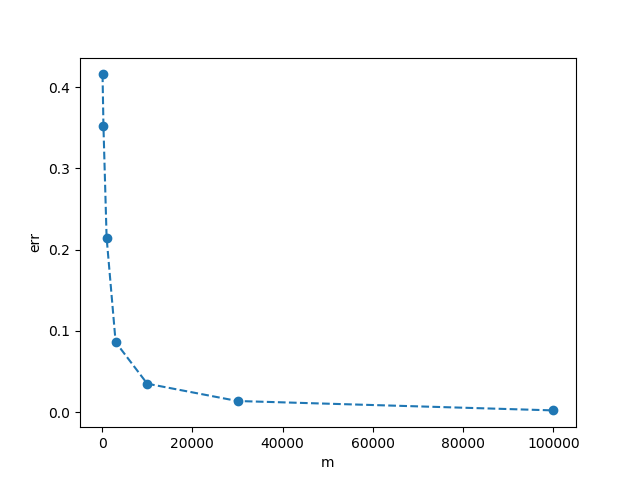
\includegraphics[width=0.7\textwidth]{q1.png}
        	\label{q1}
        	\caption{`typical' error of trees trained on $ m $ data
        		points.}
        \end{figure}
    	\par{I tested my decision trees on 50,000 underlying data points, the results are as Fig \ref{q1} shows. Generally, it is exactly what I thought it would be. As the $ m $ becomes large, the $ err $ tends to level out for the reason that the training data is large enough to allow the decision tree to see a large amount of combinations of data.}
        \item{Note that $ X $ 15 through $ X $ 20 are completely irrelevant to predicting the value of $ Y $ . For a range of $ m $ values,
        	repeatedly generate data sets of that size and fit trees to that data, and estimate the average number of
        	irrelevant variables that are included in the fit tree. How much data would you need, typically, to avoid fitting
        	on this noise?}
        \begin{figure}[H]
	        \centering
	        
\includegraphics[width=0.7\textwidth]{q2.png}
	        \label{q2}
	        \caption{Average number of irrelevant variables that are included}
	    \end{figure}
    	\par{From Fig \ref{q2} we can see 10,000 data points is not enough to eliminate the effect of irrelevant variables (Avg. no. of irrelevant variables at $ m = 100,000 $ is 4.28). Because my inelegant implementation of ID3 algorithm, I don't have enough time to test cases where $ m > 100,000 $. But I assume we would need a huge amount of data points to eliminate the effect of irrelevant variables.}
        
        \item{Generate a data set of size $ m $ = 10000, and set aside 8000 points for training, and 2000 points for testing. The
        	remaining questions should all be applied to this data set.}
        \begin{enumerate}
        	\item {\textbf{Pruning by Depth:} Consider growing a tree as a process - running ID3 for instance until all splits
        		up to depth $ d $ have been performed. Depth $ d $ = 0 should correspond to no decisions - a prediction for Y
        		is made just on the raw frequencies of $ Y $ in the data. Plot, as a function of d, the error on the training
        		set and the error on the test set for a tree grown to depth d. What does your data suggest as a good
        		threshold depth?}
        	\begin{figure}[H]
        		\centering
        		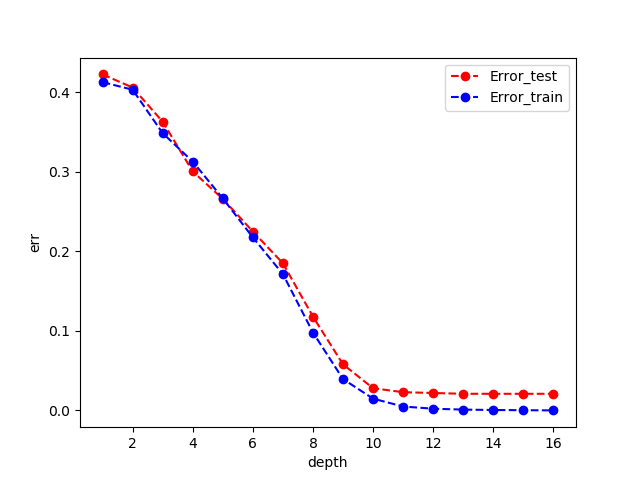
\includegraphics[width=0.7\textwidth]{q3-1.png}
        		\caption{Pruning by depth}
        		\label{q31}
        	\end{figure}
        	\par{From Fig \ref{q31} we can see, after the point $ depth = 10 $, $ err_{test} $ starts to level out while $ err_{train} $ continues to decline for a little bit. Thus, a good threshold depth could be $ depth = 10. $}
        
        	\item {\textbf{Pruning by Sample Size:} The less data a split is performed on, the less `accurate' we expect the
        		result of that split to be. Let $ s $ be a threshold such that if the data available at a node in your decision
        		tree is less than or equal to s, you do not split and instead decide $ Y $ by simple majority vote (ties broken
        		by coin flip). Plot, as a function of s, the error on the training set and the error on the testing set for a
        		tree split down to sample size s. What does your data suggest as a good sample size threshold?}
        	\begin{figure}[H]
        		\centering
        		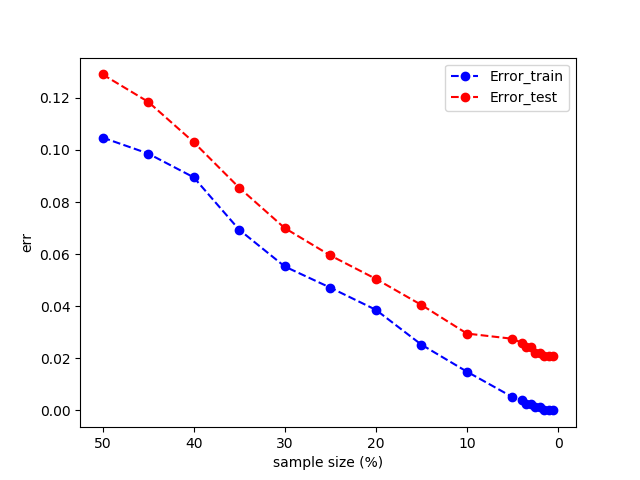
\includegraphics[width=0.7\textwidth]{q3-2.png}
        		\caption{Pruning by sample size}
        		\label{q32}
        	\end{figure}
        	\par{I did experiments on sample size of 50\%, 45\%, 40\%, 35\%, 30\%, 25\%, 20\%, 15\%, 10\%, 5\%, 4.5\%, 4\%, 3.5\%, 3\%, 2.5\%, 2\%, 1.5\%, 1\%, 0.5\% of $ m $. The results are shown in Fig \ref{q32}. We might not be able to see it very clearly from the figure. The raw data is: 0.129, 0.1185, 0.103, 0.0855, 0.07, 0.0595, 0.0505, 0.0405, 0.0295, 0.0275, 0.026, 0.0245, 0.0245, 0.022, 0.022, 0.021, 0.021, 0.021.}
        	\par{After sample size < 3\% of the size of total data points, both $ err_{train} $ and $ err_{test} $ start to level out. Thus, a good sample size threshold could be 3\% of the size of total data points.}
        
        	\item {\textbf{Pruning by Significance::} If a variable $ X $ is independent of $ Y $ , then $ X $ has no value as a splitting
        		variable. We can use something like the χ 2 -test to estimate how likely a potential splitting variable is
        		to be independent, based on the test statistic T compared to some threshold $T_0$ (in the usual 2-outcome
        		case, $T_0$ = 3.841 is used to test at a significance level of p = 5\% - see notes for more explanation). Given
        		$T_0$ , if given the data for $ X $ the value of T is less than $T_0$ , it is deemed not significant and is not used for
        		splitting. If given the data for $ X $ the value of T is greater than $T_0$ , it is deemed significant, and used for
        		splitting. Plot, as a function of $T_0$ , the error on the training set and the error on the testing set for a tree
        		split at significance threshold $T_0$ . What does your data suggest as a good threshold for significance?}
        	\begin{figure}[H]
        		\centering
        		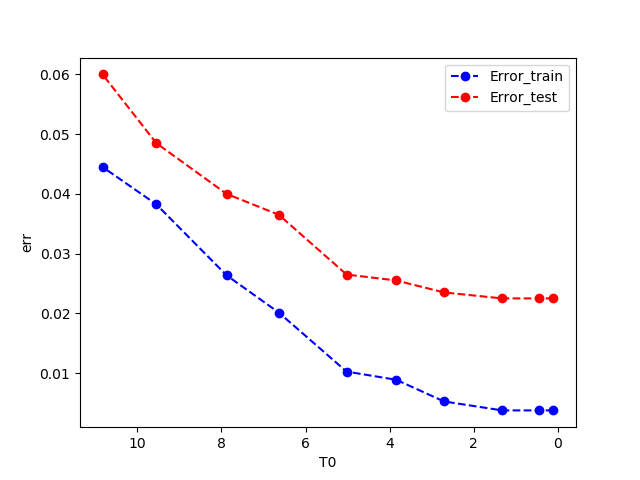
\includegraphics[width=0.7\textwidth]{q3-3.png}
        		\caption{Pruning by significance}
        		\label{q33}
        	\end{figure}
        	\par{From Fig \ref{q33} we can see, after the point $ T_0 = 3.841 $, $ err_{test} $ starts to level out while $ err_{train} $ continues to decline for a little bit. Thus, a good threshold depth could be $ T_0 = 3.841. $}
        \end{enumerate}
    
        \item{Repeat the computation of Problem 2, growing your trees only to depth $ d $ as chosen in 3.a. How does this
        	change the likelihood or frequency of including spurious variables in your trees?}
        
        \begin{figure}[H]
        	\centering
        	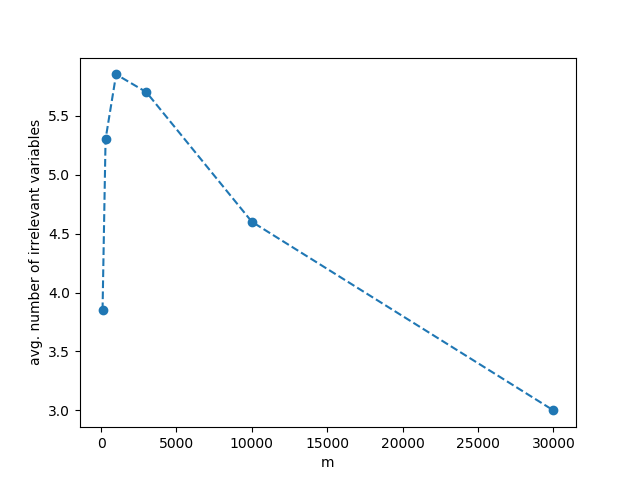
\includegraphics[width=0.7\textwidth]{q5-2.png}
        	\caption{Pruning by depth}
        	\label{q5}
        \end{figure}
        \par{From Fig \ref{q5} we can see, this change has an overall better chance of not including irrelevant variables in the fit tree, especially when $ m $ is large. This makes total sense for the reason that if we don't prune the tree, the tree would eventually start to fit on irrelevant variables. Thus by adding pruning to the tree, the likelihood of including spurious variables in my trees becomes smaller.}
        
        \item{Repeat the computation of Problem 2, splitting your trees only to sample size $ s $ as chosen in 3.b. How does
        	this change the likelihood or frequency of including spurious variables in your trees?}
        
        \begin{figure}[H]
        	\centering
        	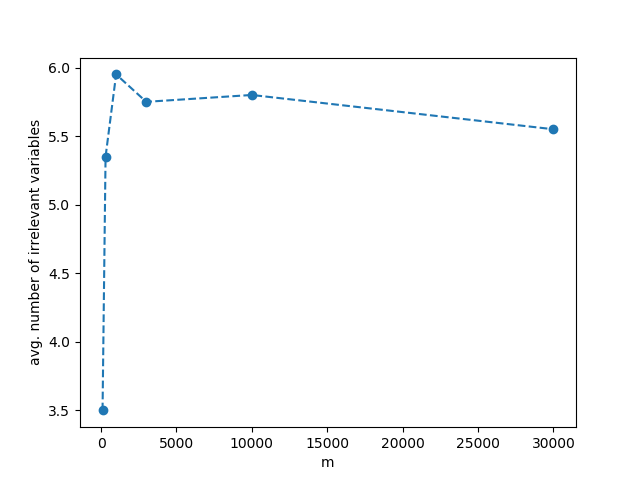
\includegraphics[width=0.7\textwidth]{q6-2.png}
        	\caption{Pruning by sample size}
        	\label{q6}
        \end{figure}
        \par{From Fig \ref{q6} we can see, this change has little improvement if not non compared to the results without pruning at all. I am actually a little surprised by this results. I guess the threshold I chose was not as good as I thought.}
        
        \item{Repeat the computation of Problem 2, splitting your trees only at or above threshold level $T_0$ as chosen in 3.c.
        	How does this change the likelihood or frequency of including spurious variables in your trees?}
        
        \begin{figure}[H]
        	\centering
        	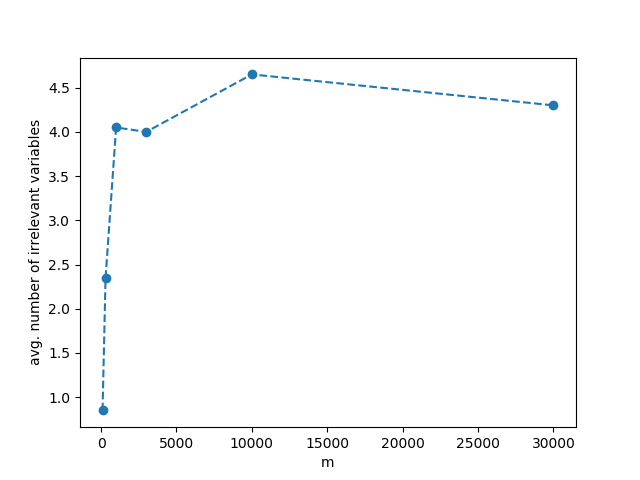
\includegraphics[width=0.7\textwidth]{q7-2.png}
        	\caption{Pruning by significance}
        	\label{q7}
        \end{figure}
        \par{From Fig \ref{q7} we can see, this change has a not bad improvement especially when $ m $ is small. This pruning method does not seem to improve much while $ m $ becomes larger. I don't have a very good explanation about this. It could be just because I didn't do enough experiments.}
        
    \end{enumerate}
\end{document}
